\chapter{绪论}

    \section{研究背景及意义}
    随着我国法治建设的逐步推进,人民的法律意识日渐提高,人们在遇到争议事件时会更多地选择诉诸法律,以公平公正地解决问题。根据最高人民法院的数据,2015年全国各级法院审结一审民事案件达622.8万件。然而,由于法律的专业性和复杂性,普通民众自身在借助法律维护自身权益的时候往往无所适从,只能求助律师等专业人士;另一方面,法律条文浩如烟海,即便是专业律师也只能专注于某一领域,在面对不熟悉的法律条文或者案例时,也需要一些决策辅助。

    信息技术,尤其是信息检索和数据挖掘技术的发展,为法律辅助系统的实现提供了可能。“北大法宝”、“找法网”等一批在线法律信息平台,提供了法规案例检索、律师推荐等功能,在一定程度上为人们诉诸法律解决争端提供了便利。然而,上述平台提供的服务并未直接解决人们的问题。法规案例的检索往往需要用户有明确的搜索目标,甚至需要一定的法律领域知识,而且即便搜索引擎能够给出相应的搜索结果,这些结果通常也无法直接解决用户的问题,需要用户自己的分析和理解。律师推荐能够方便用户找到合适的律师,实际上是连接用户和律师的桥梁,不仅无法提供问题的直接解决方案,还容易受商业化的影响,出现一些律师滥竽充数的情况。

    随着我国司法公开改革的推进以及最高人民法院关于人民法院在互联网公布裁判文书的规定的实施,蕴藏了海量信息的裁判文书可以方便地被获取和分析。2014年以来,全国各级法院共在“中国裁判文书网”上传裁判文书六百余万份,最高人民法院和部分省市区法院实现了能够上网的生效裁判文书全部上网的目标。裁判文书记载了人民法院审理案件的过程和结果,是诉讼活动结果的载体,也是人民法院确定和分配当事人实体权利义务的惟一凭证。一份结构完整、要素齐全、逻辑严谨的裁判文书,既是当事人享有权利和负担义务的凭证,也是上级人民法院监督下级人民法院民事审判活动的重要依据。因此,裁判文书中包含的当事人诉求、犯罪行为、行政执法、司法裁判行为和过程、法律的适用等信息,作为重要的历史数据,通过数据挖掘手段进行分析,可以为司法人员、律师和普通民众提供必要的决策支持。实现了一个裁判文书推荐系统,为法官提供与当前裁判文书相似的文书,作为裁判的参考。基于自然语言处理技术提取文书的语义信息,在裁判文书的相似度计算上取得了不错的效果。裁判文书推荐可以提供决策辅助,但是逐条查阅相似案例需要耗费大量精力,同时由于案例相似度不同,需要用户自行确定各个案例的权重进行综合评判,极大地降低了查询结果的直观性和明确性。

    从本质上讲,裁判是法院依照法律,对案件做出决定的过程。“以事实为根据,以法律为准绳”是我国社会主义法律适用遵循的基本原则,司法机关处理一切案件,都是根据客观事实,以国家法律为标准和尺度。因此,根据案件的描述确定适用的法律,是法院判决过程的核心部分,也是律师和普通民众在法律活动中需要解决的首要问题。运用信息技术,根据案件事实描述实现适用法律的自动识别,将在很大程度上为人们的法律活动提供更加直接和明确的帮助。现已公开的裁判文书中包含的案件事实描述以及法律适用信息,为我们提供了大量的带标签数据集,采取合适的数据挖掘手段,可以从中学习得到有效的预测模型,实现对未判案件适用法律的自动识别。


    \section{研究内容及目标}
    本文希望通过运用数据挖掘方法,从海量的裁判文书中,学习出由案件事实描述到适用法律的预测模型,从而为用户提供直接的法律决策辅助。

    一份结构完整的裁判文书包括首部、事实、理由、裁判结果和尾部五个部分,其中首部包括裁判文书的类型、编号、裁判法院,案件当事人、委托代理人等信息,事实部分包含了对案件事实的文字描述,理由部分阐述了法院对于案件的分析以及做出相应裁判结果的理由,裁判结果部分给出了法院对于此次诉讼的判决或裁定结果,尾部则包含了裁判人员、时间等信息。

    运用数据挖掘手段进行案件适用法律的自动识别,首先需要提取能够充分描述案件事实的特征,由于裁判文书及其中的事实描述部分主要是以文本形式存在,因此需要运用到文本挖掘技术对裁判文书进行处理,将其转换为结构化数据,包括中文分词,文本表示,特征选择和特征权重计算等。

    本文通过监督式学习方法来构建预测模型,样本的标签即为案件适用的法律条文,包含在裁判文书中的裁判理由部分。由于裁判文书格式的不规范性,裁判文书引用法律条文的格式没有统一格式,因此需要对提取的案件适用的法律条文作进一步处理,形成数据集的标签。与传统的分类问题不同的是,一份裁判文书中往往包含多个法律条文的引用,因此法律适用的自动识别问题是一个多标签分类问题\cite{tsoumakas2006multi}。在多标签学习中,每个样本可以对应多个标签,使得学习问题更加复杂。更进一步地,法律条文的组织呈现为树状结构,如图\ref{Figure1}所示。一个案件不仅可能适用多项法律条文,这些法律条文的具体程度也可能不同,即案件适用的法律条文可能位于树结构的叶节点,也可能位于树结构的内部节点。如果忽略法律条文的树形结构特征,无疑会损失分类标签的重要信息,造成预测模型性能的下降。因此,如何利用标签的结构信息,是本文的重要研究内容。本质上,法律适用自动识别问题是一个层次多标签学习问题\cite{barutcuoglu2006hierarchical},其中样本的特征需要通过文本挖掘手段从文本中提取,而标签的结构呈树形。

    \begin{figure}[ht]
        \centering
        % Requires \usepackage{graphicx}
        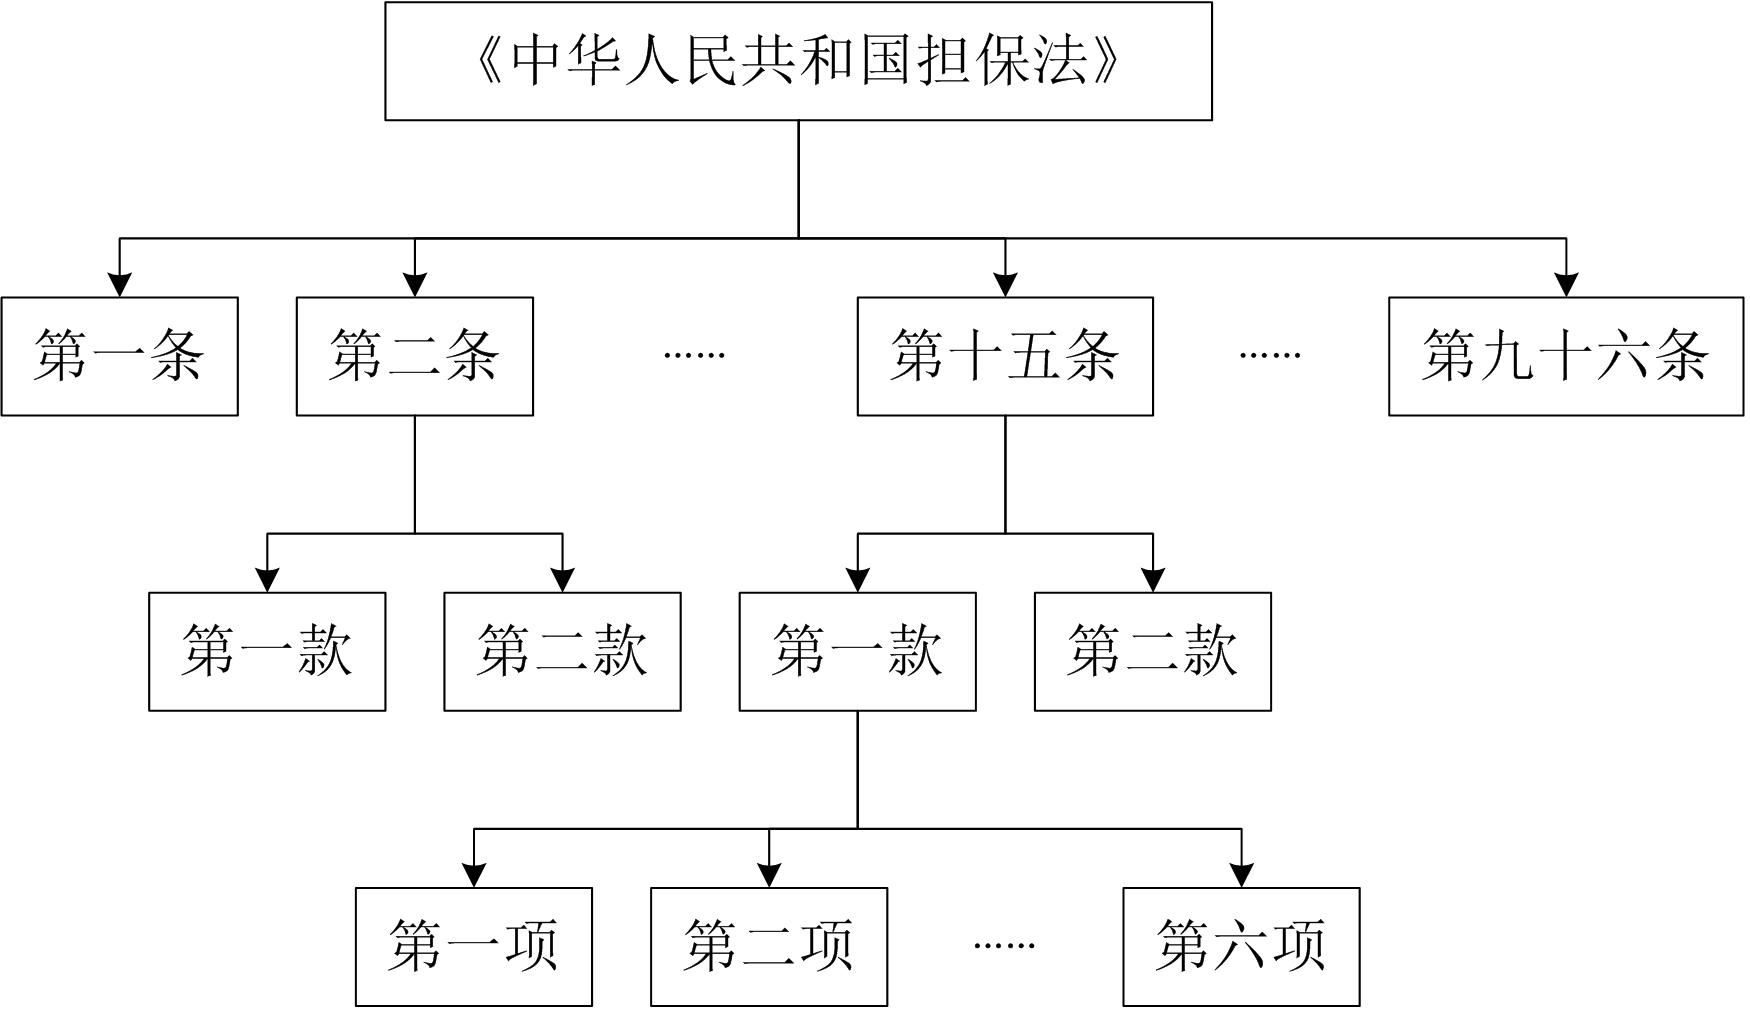
\includegraphics[width=10cm]{figures/Figure1}\\
        \caption{法律条文树形结构示例}\label{Figure1}
    \end{figure}

    综上,本文研究的目标是解决案件适用法律的自动识别问题,研究的方法是首先利用文本挖掘技术对海量裁判文书进行处理分析,得到案件事实的结构化表示,即样本特征,数据集中的每个样本可以对应于标签空间中的多个标签,标签空间以树状结构组织。在此数据集上通过层次多标签学习构建预测模型,实现对未判案件适用法律的识别。


    \section{论文组织}
    本文组织如下:

    第一章介绍本文研究的背景和意义,阐述法律适用自动识别在当前民众法律活动中的重要辅助作用,并提出研究内容和目标,指出面临的问题及解决方向。

    第二章为相关技术部分,主要对本文研究涉及的文本挖掘技术、层次多标签学习技术和非平衡分类问题进行介绍,主要对已有的层次多标签学习的工作进行综述。

    第三章详述本文提出的LocalBalance层次多标签学习算法。

    第四章为实验部分,包括本文数据集的构建,即利用文本挖掘技术对海量裁判文书进行处理,构建结构化数据集的过程,以及运用本文算法训练得到的模型的性能分析。

    第五章对本文工作进行总结,并提出改进的方向。
